 \documentclass[bachelor, och, labwork]{shiza}
% параметр - тип обучения - одно из значений:
%    spec     - специальность
%    bachelor - бакалавриат (по умолчанию)
%    master   - магистратура
% параметр - форма обучения - одно из значений:
%    och   - очное (по умолчанию)
%    zaoch - заочное
% параметр - тип работы - одно из значений:
%    referat    - реферат
%    coursework - курсовая работа (по умолчанию)
%    diploma    - дипломная работа
%    pract      - отчет по практике
% параметр - включение шрифта
%    times    - включение шрифта Times New Roman (если установлен)
%               по умолчанию выключен
\usepackage{subfigure}
\usepackage{tikz,pgfplots}
\pgfplotsset{compat=1.5}
\usepackage{float}
\usepackage{pdfpages}

\usepackage{titlesec}
\setcounter{secnumdepth}{4}
\titleformat{\paragraph}
{\normalfont\normalsize}{\theparagraph}{1em}{}
\titlespacing*{\paragraph}
{35.5pt}{3.25ex plus 1ex minus .2ex}{1.5ex plus .2ex}

\titleformat{\paragraph}[block]
{\hspace{1.25cm}\normalfont}
{\theparagraph}{1ex}{}
\titlespacing{\paragraph}
{0cm}{2ex plus 1ex minus .2ex}{.4ex plus.2ex}

% --------------------------------------------------------------------------%


\usepackage[T2A]{fontenc}
\usepackage[utf8]{inputenc}
\usepackage{graphicx}
\graphicspath{ {./images/} }
\usepackage{tempora}
\usepackage{kantlipsum}
\usepackage[sort,compress]{cite}
\usepackage{amsmath}
\usepackage{amssymb}
\usepackage{amsthm}
\usepackage{fancyvrb}
\usepackage{listings}
\usepackage{listingsutf8}
\usepackage{longtable}
\usepackage{array}
\usepackage[english,russian]{babel}

%\usepackage[colorlinks=true]{hyperref}
\usepackage{url}

\usepackage{underscore}
\usepackage{setspace}
\usepackage{indentfirst} 
\usepackage{mathtools}
\usepackage{amsfonts}
\usepackage{enumitem}
\usepackage{tikz}

\newcommand{\eqdef}{\stackrel {\rm def}{=}}
\newcommand{\specialcell}[2][c]{%
	\begin{tabular}[#1]{@{}c@{}}#2\end{tabular}}

\renewcommand\theFancyVerbLine{\small\arabic{FancyVerbLine}}

\begin{document}

	\includepdf{yahin-titulnik4.pdf}
	
	%-------------------------------------------------------------------------------------------
	\tableofcontents
	
	\newpage
	
	Цель работы — изучение основных понятий теории полугрупп.
	
	\section{Теория}
	    \subsection{Понятия полугруппы, подполугруппы и порождающего множества}

	Полугруппа – это алгебра $S = (S,\cdot)$ с одной ассоциативной бинарной операцией $\cdot$, т.е. выполняется $(x\cdot y)\cdot z = x\cdot (y\cdot z)$, $\forall x,y,z \in S$.

	Если полугрупповая операция называется умножением, то полугруппу называют мультипликативной.

	\underline{Лемма 1}. Для любого непустого множества $X$ множество всех бинарных отношений на множестве $X$ с операцией композиции является полугруппой. Такая полугруппа называется симметрической полугруппой бинарных отношений на множестве $X$ и обозначается символом $\beta(X)$.
	
	В случае конечного $n$ - элементного множества $S = {s_1,s_2,...,s_n}$ операция умножения на $S$ задаётся таблицей Кэли размерности $n \times n$, строки и столбцы которой помечены элементами множества $S$ и в которой на пересечении i–ой строки и j–го столбца стоит произведение $s_i \cdot s_j$ элементов $s_i, s_j$.
	
	\begin{figure}[H]
		\centering
		\includegraphics[width=0.7\textwidth]{keli}
		\caption{Таблица Кэли операции умножения}
		\label{fig:keli}
	\end{figure}
	
	Классификация элементов полугруппы
	
	Элемент $s$ полугруппы $S$ называется:
	
	\begin{enumerate}
		
	\item нулевым, если $s\cdot x=x\cdot s=s$ для всех $x\in S $ (при мультипликативной записи операции полугруппы такой элемент обозначается символом 0 и называется нулем);
	\item нейтральным (единичным), если $s\cdot x=x\cdot s=x$ для всех $x\in S $ (при мультипликативной записи операции полугруппы такой элемент обозначается символом 1 и называется единицей);
	\item обратимым, если для некоторого $x \in S $ выполняется свойство: $x\cdot s=s\cdot x=1$ (такой элемент x называется обратным для элемента s и обозначается символом $s^{-1}$);
	\item идемпотентом, если $s\cdot s=s$, т.е. $s^2=s$.
	
	\end{enumerate} 
	
	Если в 1) выполняется лишь равенство $x\cdot s=s$ для всех $x \in S$, то $s$ называется правым нулем. Аналогично определяется левый нуль и односторонние единицы.
	
	Подмножество $X$ полугруппы $S$ называется подполугруппой, если $X$ устойчиво относительно операции умножения, т.е. для любых $x,y \in X$ выполняется свойство: $x \cdot y \in X$.
	
	В силу общего свойства подалгебр пересечение любого семейства $X\_i (i \in I) $ подполугрупп полугруппы $S$ является подполугруппой $S$ и, значит, множество $Sub(S)$ всех подполугрупп полугруппы $S$ является системой замыканий. Следовательно, для любого подмножества $X$ полугруппы $S$ существует наименьшая подполугруппа $S$, содержащая множество $X$. Такая полугруппа обозначается символом $<X>$ и называется подполугруппой $S$, порождённой множеством $X$. При этом множество $X$ называется также порождающим множеством подполугруппы $<X>$. 
	
	В частности, если $<X> = S$, то $X$ называется порождающим множеством полугруппы $S$ и говорят, что множество $X$ порождает полугруппу $S$. 
	
	Легко видеть, что полугруппа $<X>$ состоит из всевозможных конечных произведений $x_1 \cdot ... \cdot x_n$ элементов $x_1,..., x_n \in X$ , т.е. выполняется равенство: $<X> = \{x_1 \cdot ... \cdot x_n:  n \in N $ и $x_1,..., x_n  \in X\}.$

	    \subsection{Понятия подгруппы, порождающего множества и определяющих соотношений}	
	
	 Полугруппа с единичным элементом называется моноидом. Другими словами, моноид $M = (M,\cdot ,1)$ – это алгебра с ассоциативной бинарной операцией и выделенным единичным элементом 1. При этом полугруппа $(M,\cdot)$ называется полугруппой моноида $M = (M,\cdot ,1)$.
	 
	Для любой полугруппы $S = (S,\cdot)$ канонически определяется моноид $M(S)$ по следующему правилу: $M(S) = S \cup {1} $ для некоторого элемента $1\notin S$ и умножение в $M(S)$ на новый элемент 1 определяется по формуле: $x \cdot 1=1 \cdot x = x$. Полугруппа моноида $M(S)$ обозначается символом $S^1$ и называется полугруппой с внешне присоединенной единицей.
	
	Моноид называется группой, если в нем все элементы обратимы.
	
	\underline{Лемма}. Для любого моноида M множество всех обратимых элементов $M^*$ с операцией умножения моноида является группой, т.е. для любых $a,b \in M^*$  выполняется условие $a \cdot b \in M^*$
	
	Подгруппой полугруппы $S$ назовем подполугруппу $T$ из $S$, являющуюся группой относительно бинарной операции, определенной в $S$. Это эквивалентно тому, что $T$ есть подполугруппа из $S$, в которой для любых $a,b \in T$ существуют $x,y \in T$ такие, что $ax=b$ и $ya=b$. Отсюда легко получить, что подмножество $T$ полугруппы $S$ является подгруппой тогда и только тогда, когда $aT=Ta=T$ для любого $a \in T$.
	
	Единица $e$ подгруппа $T$ полугруппы $S$ является идемпотентом, но не обязательно единицей полугруппы $S$.
	
	Пусть $A$ – произвольное множество, называемое алфавитом. Элементы $a \in A$ называются буквами. Словом над алфавитом $A$ называется конечная последовательность букв $a_1,...,a_n$ алфавита $A$.
	
	Обозначим символом $A^+$ множество всех непустых слов над алфавитом и символом $A^*$ - множество слов $A^* = A^+ \cup {\land}$.
	
	\underline{Теорема (О представлении полугрупп словами)}. Любая полугруппа $S$ является фактор-полугруппой некоторой полугруппы слов $A^+$, т.е. $S \cong A/\epsilon$ для некоторой конгруэнции $\epsilon$ полугруппы $A^+$.
	
	Таким образом, для любой конечной полугруппы $S$ найдется такой конечный алфавит $A$, что для некоторого отображения $\phi:A \to S$ выполняется равенство $< \phi(A) \geq S$ и, значит, $S \cong A^+/ker f$. В этом случае множество $A$ называется множеством порождающих символов полугруппы $S$ (относительно отображения $\phi: A \to S$).
	
	Если при этом для слов $w_1,w_2  \in A^+$ выполняется равенство $\phi(w_1)=\phi(w_2)$, т.е. $w_1 \equiv w_2 (ker \phi )$, то говорят, что на S выполняется соотношение $w_1=w_2$ (относительно отображения $\phi:A \to S$ ).
	
	Очевидно, что в общем случае множество таких соотношений $w_1  = w_2$ для всех пар $(w_1, w_2)\in ker \phi$ будет бесконечным и не представляется возможности эффективно описать полугруппу $S$ в виде полугруппы классов конгруэнции $ker \phi$. Однако в некоторых случаях можно выбрать такое сравнительно простое подмножество $\rho \subset ker \phi$, которое однозначно определяет конгруэнцию $ker \phi$ как наименьшую конгруэнцию полугруппы $A^+$, содержащую отношение $\rho$, т.е. $ker \rho \phi = f_{con} (\rho)=f_{eq} (f_{reg} (\rho))$.
	
	Так как в случае $(w_1,w_2) \in \rho$ по-прежнему выполняется равенство $\phi(w_1)=\phi(w_2)$, то будем писать $w_1=w_2$ и называть такие выражения определяющими соотношениями.

	\section{Результаты работы}
	
	\subsection{Алгоритм построения подполугрупп по таблице Кэли}
	
	$\textit{Вход:}$ Полугруппа $S$ с таблицей Кэли и подмножество $X \subset S$.

	$\textit{Выход:}$  Подполугруппа $<X> \subset S$.

	\begin{enumerate} 
		\item Положим $i = 0, X_0 = X$;
		\item Для $X_i$ вычислим $\overline{X_l} = {x \cdot y : x \in X_i \wedge y \in X}$ и положим $X_{i+1} = X_i \cup \overline{X_l}$.
		\item Вычисляем $<X> = \bigcup_{i=0}^{\infty} X_i$.
	\end{enumerate} 
	
	Временная сложность алгоритма построения подполугрупп по таблице Кэли = $O(n^2 * m)$, где $m$ - количество элементов в подмножестве X, а n - это размер множества для полугруппы S.
	
	\subsection{Алгоритм построения полугруппы бинарных отношений по заданному порождающему множеству}
	
	$\textit{Вход:}$ Конечное множество множество $X$ бинарных отношений (булевых матриц).
	
	$\textit{Выход:}$  Полугруппа $<X>$, таблица Кэли операции умножения матриц из $<X>$.
	
	\begin{enumerate} 
		\item Пока не будет добавлена ни одна новая матрица за весь цикл, выполняется:
		\begin{enumerate} 
			\item Запускается цикл for с g\_now от 0 до размера списка матриц res\_all\_matr, который обходит все матрицы из res\_all\_matr и в нем запускается еще один цикл for с g от 0 до размера списка матриц res\_all\_matr.
				\begin{enumerate} 
						\item Создается матрица с нулевыми элементами  matrix\_res
						\item Если g\_now[i][k] == 1 и  g[k][j] == 1, то в результирующей матрице matrix\_res[i][j] присваивается 1.
						\item Если полученной матрицы matrix\_res еще нет в res\_all\_matr, то она вносится туда.
				\end{enumerate}
		\end{enumerate}
		\item Возвращается res\_all\_matr и таблица Кэли операции умножения матриц из res\_all\_matr.
	\end{enumerate} 
	
	Временная сложность алгоритма построения полугруппы бинарных отношений по заданному порождающему множеству = $O(m^2 * n^3 * p)$, где n - это размерность матриц, m - количество матриц в res\_all\_matr, а p - число раз, когда в цикле находилась хотя бы одна новая матрица
	
	\subsection{Алгоритм построения полугруппы по порождающему множеству и определяющим соотношениям}
	
	$\textit{Вход:}$ Конечное множество символов $A$ и конечное множество $R$ определяющих соотношений.
	
	$\textit{Выход:}$  Полугруппа $<A|R>$, таблица Кэли операции умножения слов из $<A|R>$.
	
	\begin{enumerate} 
		\item Создается полная система представителей $<A|R>$, т.е. список, куда будут заноситься слова, эквивалентные относительно конгруэнции $\epsilon$ ранее занесенным туда словам.
		\item Все слова из конечного множества символов $A$ вносятся в $<A|R>$.
		\item Пока все слова, полученные в цикле не будут эквивалентны относительно конгруэнции $\epsilon$ словам из $<A|R>$, выполняется: 
		\begin{enumerate} 
			\item Рассматриваются все слова w, полученные умножением справа элементов конечного множества символов $A$ к внесенным в $<A|R>$ на предыдущем шаге словам. К каждому из полученных слов применяются преобразования $R$ до того момента, когда не подойдет ни одно из определяющих соотношений. 
			\item Если полученное на шаге 3 слово не эквивалентно относительно конгруэнции $\epsilon$ словам из $<A|R>$, то это слово кладется в $<A|R>$.
		\end{enumerate} 
	\item Возвращаются $<A|R>$ и таблица Кэли операции умножения слов из $<A|R>$.
	\end{enumerate} 

	Временная сложность алгоритма построения полугруппы по порождающему множеству и определяющим соотношениям = $O(m^2 * n^2 * p)$, где m - размер конечного множества $R$, n - длина слова, а  p - максимальная длина слова.

	\section{Код программы}		
	
	 \begin{verbatim}
	 	
#include <iostream>
#include <vector>
#include <math.h>
#include <algorithm>
#include <string>
#include <iomanip>

using namespace std;

int CharInt(int N, char c, vector <char> mnojestvo) {
	for (int i = 0; i < N; i++)
	{
		if (mnojestvo[i] == c)
		return i;
	}
}

bool proverka_Ass(int N, char** keli, vector <char> mnojestvo) {
	bool prov = true;
	for (int x = 0; x < N; x++)
	{
		for (int y = 0; y < N; y++)
		{
			for (int z = 0; z < N; z++)
			{
				if (keli[x][CharInt(N, keli[y][z], mnojestvo)] 
				!= keli[CharInt(N, keli[x][y], mnojestvo)][z])
				prov = false;
			}
		}
	}
	return prov;
}

bool true_elems(vector <char> X_i, vector <char> X_i_next) {
	if (X_i.size() != X_i_next.size())
	return true;
	else {
		for (int j = 0; j < X_i.size(); j++) {
			if (X_i[j] != X_i_next[j])
			return true;
		}
	}
	return false;
}

bool unique_elem(vector <char> ch, char elem) {
	for (int j = 0; j < ch.size(); j++) {
		if (elem == ch[j])
		return false;
	}
	return true;
}

void postr_podpol(int N, vector <char> mnojestvo, int M, 
vector <char> X, char** keli) {
	int i = 0;
	vector <char> X_i;
	vector <char> X_i_next;
	vector <char> X_dop;
	vector <char> X_res;
	for (int j = 0; j < M; j++) {
		X_i.push_back(X[j]);
		X_res.push_back(X[j]);
		X_i_next.push_back(X[j]);
	}
	for (int j = 0; j < X_i.size(); j++) {
		for (int k = 0; k < X_i.size(); k++) {
			char x_y = keli[CharInt(N, X_i[j], mnojestvo)]
			[CharInt(N, X_i[k], mnojestvo)];
			if (unique_elem(X_dop, x_y)) {
				X_dop.push_back(x_y);
			}
		}
	}
	for (int j = 0; j < X_dop.size(); j++) {
		if (unique_elem(X_res, X_dop[j])) {
			X_res.push_back(X_dop[j]);
		}
		if (unique_elem(X_i_next, X_dop[j])) {
			X_i_next.push_back(X_dop[j]);
		}
	}
	
	int sch = 1;
	while (true_elems(X_i, X_i_next) || sch == 1) {
		sch = 0;
		X_i.clear();
		for (int j = 0; j < X_i_next.size(); j++) {
			X_i.push_back(X_i_next[j]);
		}
		X_dop.clear();
		for (int j = 0; j < X_i.size(); j++) {
			for (int k = 0; k < X_i.size(); k++) {
				int x_y = keli[CharInt(N, X_i[j], mnojestvo)]
				[CharInt(N, X_i[k], mnojestvo)];
				if (unique_elem(X_dop, x_y)) {
					X_dop.push_back(x_y);
				}
			}
		}
		for (int j = 0; j < X_dop.size(); j++) {
			if (unique_elem(X_i_next, X_dop[j])) {
				X_i_next.push_back(X_dop[j]);
			}
		}
		for (int j = 0; j < X_i_next.size(); j++) {
			if (unique_elem(X_res, X_i_next[j])) {
				X_res.push_back(X_i_next[j]);
			}
		}
		sort(X_res.begin(), X_res.end());
		if (X_res.size() == N) {
			for (int j = 0; j < X_res.size(); j++) {
				cout << X_res[j] << ", ";
			}
			return;
		}
	}
	for (int j = 0; j < X_res.size(); j++) {
		cout << X_res[j] << ", ";
	}
	return;
}

void proverka_1(int N, vector <char> mnojestvo, int M, 
vector <char> podmnojestvo, char** keli) {
	
	cout << endl;
	if (proverka_Ass(N, keli, mnojestvo) == true) {
		postr_podpol(N, mnojestvo, M, podmnojestvo, keli);
	}
	else
	cout << "Не ассоциативна" << endl;
	
}

bool unique_matr(vector < vector <int> >matrix_res, 
vector < vector < vector <int> > > res_all_matr) {
	for (int i = 0; i < res_all_matr.size(); i++)
	{
		if (matrix_res == res_all_matr[i])
		return false;
	}
	return true;
}
int mult_matr(vector < vector <int> > matrix1, 
vector < vector <int> > matrix2, int N, 
vector < vector < vector <int> > > res_all_matr) {
	vector < vector <int> >  matrix_res;
	vector <int> s(N, 0);
	for (int jh = 0; jh < N; jh++)
	{
		matrix_res.push_back(s);
	}
	for (int i = 0; i < N; i++)
	{
		for (int j = 0; j < N; j++)
		{
			for (int k = 0; k < N; k++) {
				if (matrix1[i][k] == 1 && matrix2[k][j] == 1) {
					matrix_res[i][j] = 1;
					break;
				}
			}
		}
	}
	for (int g = 0; g < res_all_matr.size(); g++)
	{
		if (matrix_res == res_all_matr[g])
		return g + 1;
		//cout << setw(6) << "№" << g + 1 << " ";
	}
}
void second_bin(int N, vector < vector < vector <int> > > res_all_matr, 
int matr_count) {
	int razmer = res_all_matr.size();
	int dps = 0;
	while (res_all_matr.size() != razmer || dps == 0) {
		razmer = res_all_matr.size();
		dps = 1;
		for (int g_now = 0; g_now < razmer; g_now++)
		{
			for (int g = 0; g < razmer; g++)
			{
				vector < vector <int> >  matrix_res;
				vector <int> s(N, 0);
				for (int jh = 0; jh < N; jh++)
				{
					matrix_res.push_back(s);
				}
				for (int i = 0; i < N; i++)
				{
					for (int j = 0; j < N; j++)
					{
						for (int k = 0; k < N; k++) {
							if (res_all_matr[g_now][i][k] == 1 
							&& res_all_matr[g][k][j] == 1) {
								matrix_res[i][j] = 1;
								break;
							}
						}
					}
				}
				if (unique_matr(matrix_res, res_all_matr)) {
					res_all_matr.push_back(matrix_res);
				}
			}
		}
	}
	cout << "Получаем: " << endl;
	for (int g = 0; g < res_all_matr.size(); g++)
	{
		cout << "Матрица " << g + 1 << endl;
		for (int i = 0; i < N; i++) {
			for (int j = 0; j < N; j++) {
				cout << res_all_matr[g][i][j] << " ";
			}
			cout << endl;
		}
		cout << endl;
		cout << endl;
	}
	
	cout << "Таблица Кэли: " << endl;
	cout << setw(6) << " " << " ";
	for (int i = 0; i < res_all_matr.size(); i++) {
		cout << setw(6) << i + 1;
	}
	int s_d = 0;
	cout << endl;
	for (int g = 0; g < res_all_matr.size(); g++)
	{
		cout << setw(6) << g + 1 << " ";
		for (int f = 0; f < res_all_matr.size(); f++)
		{
			cout << setw(6) << mult_matr(res_all_matr[g], 
			res_all_matr[f], N, res_all_matr);
		}
		cout << endl;
	}
}

bool unique_word(string A_i, vector <string> s_predst) {
	for (int i = 0; i < s_predst.size(); i++)
	{
		if (A_i == s_predst[i])
		return false;
	}
	return true;
}

bool unique_word_on_pair(string word, 
vector < pair < string, string > > relations, string& sec_pair) {
	for (int i = 0; i < relations.size(); i++)
	{
		if (word == relations[i].first) {
			sec_pair = relations[i].second;
			return false;
		}
	}
	return true;
}

vector<string> word_vector(string word)
{
	vector<string> convert_word;
	for (int i = 0; i < word.size(); ++i)
	convert_word.push_back(word.substr(i, 1));
	
	return(convert_word);
}

vector <string> res_keli_elems;

void find_res_word(string keli_word, vector <string> S, 
vector < pair < string, string > > relations, 
int max_w, int max_sist_pred);

bool dop_proverka(string keli_word, vector <string> S, 
vector < pair < string, string > > relations, int max_w,
 int max_sist_pred) {
	int start_size = res_keli_elems.size();
	find_res_word(keli_word, S, relations, max_w, max_sist_pred);
	
	if (start_size != res_keli_elems.size()) {
		if (res_keli_elems.size() == 1 ||
		 res_keli_elems[res_keli_elems.size() - 1] 
		== res_keli_elems[res_keli_elems.size() - 2]) {
			if (res_keli_elems.size() != 1) {
				res_keli_elems.erase(res_keli_elems.begin() +
				 res_keli_elems.size() - 1);
			}
			return true;
		}
		return false;
	}
	return true;
}

void find_res_word(string keli_word, vector <string> S, 
vector < pair < string, string > > relations, int max_w, int max_sist_pred) {
	if (!unique_word(keli_word, S)) {
		//cout << keli_word << " ";
		res_keli_elems.push_back(keli_word);
		return;
	}
	else {
		string rec_word;
		vector<string> word_now = word_vector(keli_word);
		
		int sch = 2;
		while (sch <= max_w)
		{
			for (int i = word_now.size() - 1; i >= 0; --i)
			{
				if (sch > keli_word.size() || sch > i + 1)
				break;
				int j;
				string f_part = "";
				for (j = i; j > i - sch; --j)
				f_part = word_now[j] + f_part;
				string s_pair = "";
				if (!unique_word_on_pair(f_part, relations, s_pair))
				{
					rec_word = "";
					vector<string> part_ = word_vector(s_pair);
					
					for (int k = 0; k < j + 1; ++k)
					rec_word = rec_word + word_now[k];
					
					rec_word = rec_word + s_pair;
					
					for (int k = i + 1; k < word_now.size(); ++k)
					rec_word = rec_word + word_now[k];
					
					if (rec_word.size() < keli_word.size())
					{
						res_keli_elems.push_back(rec_word);
						if (dop_proverka(rec_word, S, relations, max_w,
						 max_sist_pred)) {
							//cout << rec_word << " ";
							return;
						}
						else
						find_res_word(rec_word, S, relations, max_w, max_sist_pred);
					}
					else
					find_res_word(rec_word, S, relations, max_w, max_sist_pred);
				}
			}
			sch++;
		}
	}
}

void vivod_keli(vector <string> S, 
vector < pair < string, string > > relations, 
int max_w, int max_sist_pred) {
	cout << endl;
	cout << "Операция умножения таких слов определяется по следующей 
	таблице Кэли : " << endl;
	cout << setw(6) << " " << " ";
	for (int i = 0; i < S.size(); i++)
	{
		cout << setw(6) << S[i] << " ";
	}
	cout << endl;
	for (int i = 0; i < S.size(); i++)
	{
		cout << setw(6) << S[i] << " ";
		for (int j = 0; j < S.size(); j++)
		{
			string keli_word = S[i] + S[j];
			find_res_word(keli_word, S, relations, max_w, max_sist_pred);
			cout << setw(6) << res_keli_elems[res_keli_elems.size() - 1] << " ";
			res_keli_elems.clear();
		}
		cout << endl;
	}
}

vector <string> S;

void th_alg(string& word, vector <string>& A_ofr, 
int& max_w, string& new_word, 
string& rec_word, vector < pair < string, string > >& relations)
{
	if (!unique_word(word, A_ofr))
	return;
	
	vector<string> word_now = word_vector(word);
	
	int sch = 2;
	while (sch <= max_w)
	{
		for (int i = word_now.size() - 1; i >= 0; --i)
		{
			if (sch > word.size() || sch > i + 1)
			break;
			int j;
			string f_part = "";
			for (j = i; j > i - sch; --j)
			f_part = word_now[j] + f_part;
			string s_pair = "";
			if (!unique_word_on_pair(f_part, relations, s_pair))
			{
				rec_word = "";
				vector<string> part_ = word_vector(s_pair);
				
				for (int k = 0; k < j; ++k)
				rec_word = rec_word + word_now[k];
				
				rec_word = rec_word + s_pair;
				
				for (int k = i + 1; k < word_now.size(); ++k)
				rec_word = rec_word + word_now[k];
				
				if (rec_word.size() < word.size())
				{
					A_ofr.push_back(word);
					A_ofr.push_back(rec_word);
					return;
				}
				else if (!unique_word(rec_word, A_ofr))
				return;
				else {
					th_alg(rec_word, A_ofr, max_w, new_word, rec_word, relations);
				}
			}
			if (!unique_word(word, A_ofr))
			return;
		}
		sch++;
	}
	
	if (rec_word.size() == word.size() && rec_word < word 
	&& unique_word(word, A_ofr) && unique_word(rec_word, A_ofr))
	{
		S.push_back(rec_word);
		A_ofr.push_back(word);
		A_ofr.push_back(rec_word);
		return;
	}
	
	S.push_back(word);
	A_ofr.push_back(word);
	A_ofr.push_back(rec_word);
	return;
}

int main()
{
	setlocale(LC_ALL, "Rus");
	vector <char> mnojestvo;
	vector <char> podmnojestvo;
	vector <string> A;
	vector <string> A_ofr;
	vector < vector < vector <int> > > all_matr;
	vector < vector < vector <int> > > res_all_matr;
	int sposob, i, j, N, M, T, matr_count, R_count, R;
	int max_w = 0;
	cout << "Введите, что хотите сделать: " << endl;
	cout << "1 - построение подполугрупп по таблице Кэли" << endl;
	cout << "2 - построение полугруппы бинарных отношений по заданному 
	порождающему множеству" << endl;
	cout << "3 - построение полугруппы по порождающему множеству и 
	определяющим соотношениям" << endl;
	cin >> sposob;
	
	if (sposob == 1)
	{
		
		cout << "Введите размерность полугруппы: " << endl;
		cin >> N;
		if (N == 0) {
			cout << "Ошибка";
			return 0;
		}
		cout << "Введите множество для полугруппы S: " << endl;
		char vv;
		for (int i = 0; i < N; i++) {
			cin >> vv;
			mnojestvo.push_back(vv);
		}
		char** keli;
		keli = new char* [N];
		cout << "Таблица Кэли полугруппы S: " << endl;
		for (int i = 0; i < N; i++) {
			keli[i] = new char[N];
			for (int j = 0; j < N; j++) {
				cin >> keli[i][j];
			}
		}
		cout << "Введите размерность подмножества: " << endl;
		cin >> M;
		if (M == 0) {
			cout << "Ошибка";
			return 0;
		}
		cout << "Введите подмножество X: " << endl;
		char podvv;
		for (int i = 0; i < M; i++) {
			cin >> podvv;
			podmnojestvo.push_back(podvv);
		}
		proverka_1(N, mnojestvo, M, podmnojestvo, keli);
	}
	else if (sposob == 2)
	{
		cout << "Введите размерность : " << endl;
		cin >> N;
		if (N == 0) {
			cout << "Ошибка";
			return 0;
		}
		cout << "Количество матриц : " << endl;
		cin >> matr_count;
		if (matr_count == 0) {
			cout << "Ошибка";
			return 0;
		}
		for (int l = 0; l < matr_count; l++)
		{
			cout << "Введите матрицу бинарного отношения №" 
			<< l + 1 << ": " << endl;
			vector < vector <int> > matrix1(N);
			for (int i = 0; i < N; i++) {
				for (int j = 0; j < N; j++) {
					int vvod_ch;
					cin >> vvod_ch;
					matrix1[i].push_back(vvod_ch);
				}
			}
			res_all_matr.push_back(matrix1);
		}
		
		second_bin(N, res_all_matr, matr_count);
	}
	else if (sposob == 3) {
		cout << "Введите количество символов в алфавите A: " << endl;
		int T;
		cin >> T;
		cout << "Введите конечное множество символов А (алфавит): " << endl;
		string vvod_A;
		for (int i = 0; i < T; i++) {
			cin >> vvod_A;
			A.push_back(vvod_A);
			S.push_back(vvod_A);
			A_ofr.push_back(vvod_A);
		}
		cout << "Введите количество пар в определяющем соотношении R: " << endl;
		int R_count;
		cin >> R_count;
		vector < pair < string, string > > relations;
		relations.resize(R_count);
		cout << "Введите определяющее соотношение R (так: R1 R2): " << endl;
		for (int i = 0; i < R_count; i++) {
			string vvod_R1;
			string vvod_R2;
			cin >> vvod_R1 >> vvod_R2;
			if (vvod_R1.size() > max_w)
			max_w = vvod_R1.size();
			if (vvod_R2.size() > max_w)
			max_w = vvod_R2.size();
			if (vvod_R1.size() < vvod_R2.size())
			relations.push_back(make_pair(vvod_R2, vvod_R1));
			else if (vvod_R1.size() > vvod_R2.size())
			relations.push_back(make_pair(vvod_R1, vvod_R2));
			else
			{
				if (vvod_R1 < vvod_R2)
				relations.push_back(make_pair(vvod_R2, vvod_R1));
				else
				relations.push_back(make_pair(vvod_R1, vvod_R2));
			}
		}
		int len = 1;
		vector <string>  dop_A;
		dop_A = A;
		string new_word;
		string rec_word;
		while (!dop_A.empty())
		{
			++len;
			for (int i = 0; i < dop_A.size(); i++)
			{
				string word_w = dop_A[i];
				for (int i = 0; i < A.size(); i++)
				{
					string let = A[i];
					string word_w_let = word_w + let;
					rec_word = "";
					th_alg(word_w_let, A_ofr, max_w, new_word, rec_word, relations);
				}
			}
			dop_A.clear();
			for (int i = 0; i < S.size(); i++)
			{
				if (S[i].size() == len)
				dop_A.push_back(S[i]);
			}
		}
		
		cout << "Полная система представителей: S = { ";
			for (int i = 0; i < S.size(); i++)
			{
				cout << S[i] << " ";
			}
			cout << " }" << endl;
		int max_sist_pred = 0;
		for (int i = 0; i < S.size(); i++)
		{
			if (S[i].size() > max_sist_pred)
			max_sist_pred = S[i].size();
		}
		vivod_keli(S, relations, max_w, max_sist_pred);
	}
	else
	cout << "Ошибка" << endl;
	
	cout << endl;
}
	
	\end{verbatim}
	
	\section{Результаты тестирования программ}
	
	Тестирование №1:
	
Построение подполугрупп по таблице Кэли.

	\begin{figure}[H]
		\centering
		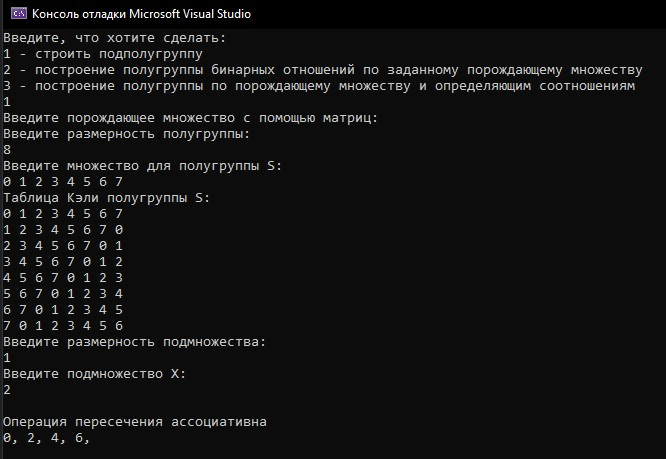
\includegraphics[width=0.9\textwidth]{test_1}
		\caption{Тестировние №1}
		\label{fig:test_1}
	\end{figure}
	
	Тестирование №2:
	
Построение полугруппы бинарных отношений по заданному порождающему множеству.
	
	\begin{figure}[H]
		\centering
		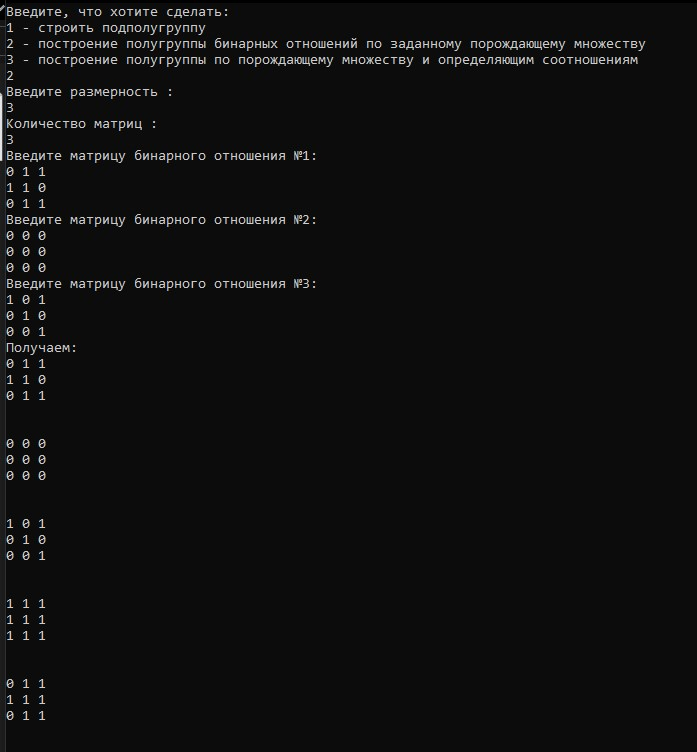
\includegraphics[width=0.9\textwidth]{test_2}
		\caption{Тестировние №2}
		\label{fig:test_2}
	\end{figure}
	
	Тестирование №3:

Построение полугруппы по порождающему множеству и определяющим соотношениям.

	
	\begin{figure}[H]
		\centering
		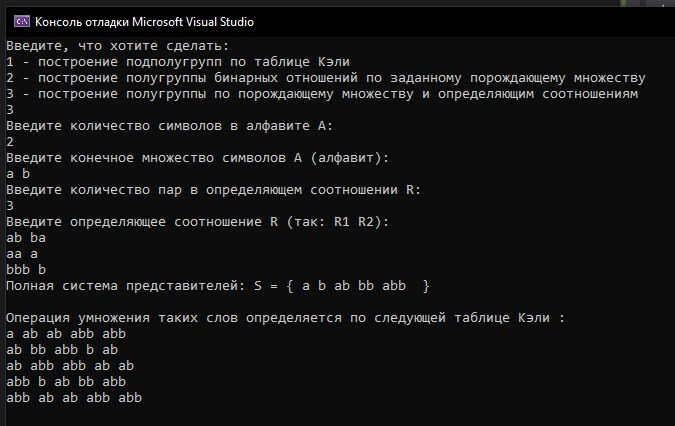
\includegraphics[width=0.9\textwidth]{test_3}
		\caption{Тестировние №3}
		\label{fig:test_3}
	\end{figure}
	
	\newpage
	\conclusion %заключение
	
	В данной лабораторной работе были рассмотрены и изучены следующие темы: понятия полугруппы, подполугруппы и порождающего множества, понятия подгруппы, порождающего множества и определяющих соотношений. Во второй части работы были реализованы: алгоритм построения подполугрупп по таблице Кэли, алгоритм построения полугруппы бинарных отношений по заданному порождающему множеству, алгоритм построения полугруппы по порождающему множеству и определяющим соотношениям.  
	  
	
	
	
\end{document}